\section{Use Cases}
\label{uc:sec:use_cases}

\begin{itemize}
	\item \textbf{Ziel}: Requirements in Text- und Diagramm-Form festhalten und visualisieren
	\item Use Cases beschreiben eine \textbf{Interaktion} mit einem System und dessen \textbf{Verhalten}
	\item \textbf{Diagrammelemente}:
	\begin{itemize}
		\item \textbf{Actors}, visualisiert als Strichmännchen links vom System
		\item \textbf{Scopes}, welche das System und die Umgebung abgrenzen (z.B Versicherungsfirma und ein bestimmter Service Desk), visualisiert als Kästen um das System
		\item \textbf{Interaktionen}: Durchzuführende Interaktionen, visualisiert als eingekreisten Text
		\item ggf. \textbf{Supporting Actors}, visualisiert als Kasten rechts vom System
	\end{itemize}
	\item \textbf{Weitere Terminologie}:
	\begin{itemize}
		\item \textbf{Stakeholder} sind Personen oder Organisationen mit indirektem Einfluss aufgrund von berechtigtem Interesse (z.B Aktieninhaber)
		\item Der \textbf{Primary Actor} initiiert die Interaktion
		\item Das \textbf{Use Case Model} ist die Menge aller zusammengehörigen Use Cases
		\item Eine spezifische Folge von Aktionen und Interaktionen wird \textbf{Szenario} genannt
	\end{itemize}
	\item \textbf{Gebräuchliche Scopes}:
	\begin{itemize}
		\item \textbf{Business Use Case} für eine gesamte Firma
		\item \textbf{System Use Case} für das eigentliche System
		\item \textbf{Component Use Case} für eine einzelne Komponente des Systems
	\end{itemize}
	\item Granularität eines Use Cases oft unklar, deshalb: Orientierung an \textbf{Elementary Business Processes (EBPs)}:
	\begin{itemize}
		\item Ein \textbf{einzelner} Task, der von \textbf{einer} Person an \textbf{einer} Stelle zu \textbf{einer bestimmten Zeit} durchgeführt wird
		\item Dieser Task hat \textbf{messbaren Wert} für das Unternehmen und hinterlässt alle Daten in einem \textbf{konsistenten Zustand}
	\end{itemize}
	\item Unterscheide \textbf{Goal Levels}:
	\begin{itemize}
		\item (High-Level) \textbf{Summary}: Vereinigt niedrigere Goal Levels (meist) zu einem Business Use Case
		\item \textbf{User Goal}: Äquivalent zu einem EBP, beschreibt Nutzerinteraktion mit dem System
		\item \textbf{Subfunction}: Nähere Ausführung der Interaktionen in User Goals
	\end{itemize}
	\item Use Cases definiert und verfeinert man am besten \textbf{iterativ}, ggf. mit Orientierung an einer Struktur wie
	\begin{itemize}
		\item \textbf{Fully Dressed} (siehe unten)
		\item \textbf{Casual} (oft keine bestimmte Struktur, plain text)
		\item \textbf{One-Column-Table / Two-Column-Tables} (Fully Dressed in Tabellenform, ggf. mit einer Spalte für Actor, einer für System)
		\item \textbf{RUP Style} (ähnlich zu Fully Dressed)
	\end{itemize}
\end{itemize}

\subsection{Fully Dressed Style}
\label{uc:sub:fully_dressed_style}

\begin{enumerate}
	\item \textbf{Preface Elements}: Viele optionale Elemente, oft Beschreibung des Primary Actors
	\item \textbf{Stakeholders and Interest List}: Was \textbf{muss} das System erfüllen? \textbf{Wer} benötigt dies?
	\item \textbf{Preconditions}: Voraussetzungen, damit der Use Case überhaupt \textbf{durchführbar} ist
	\item \textbf{Postconditions}: Voraussetzungen, sodass der Use Case als \textbf{abgeschlossen} gelten kann
	\item \textbf{Main Success Scenario}: \textbf{Bestmögliches} Szenario
	\item \textbf{Extensions}: Interessante \textbf{Alternativpfade} zu Erfolg oder Fehlschlag
	\item \textbf{Special Requirements}: Relevante \textbf{nicht-funktionale} Requirements
	\item \textbf{Technology and Data Variations}: z.B gerätespezifische Probleme und damit einhergehende Variationen
\end{enumerate}

\subsection{Software Requirements Specification}
\label{uc:sub:software_requirements_specification}

\begin{itemize}
	\item Beschreibung des \textbf{externen Verhaltens} der Software
	\item Dokumentation aller \textbf{Interfaces} zwischen Software und Environment (System selbst ist \textbf{Black Box})
	\item \textbf{Form}: Introduction, Overall Description, Requirements, Appendix, Index
\end{itemize}

\subsection{Beispiel}
\label{uc:sub:beispiel}

\begin{figure}[!h]
	\centering
	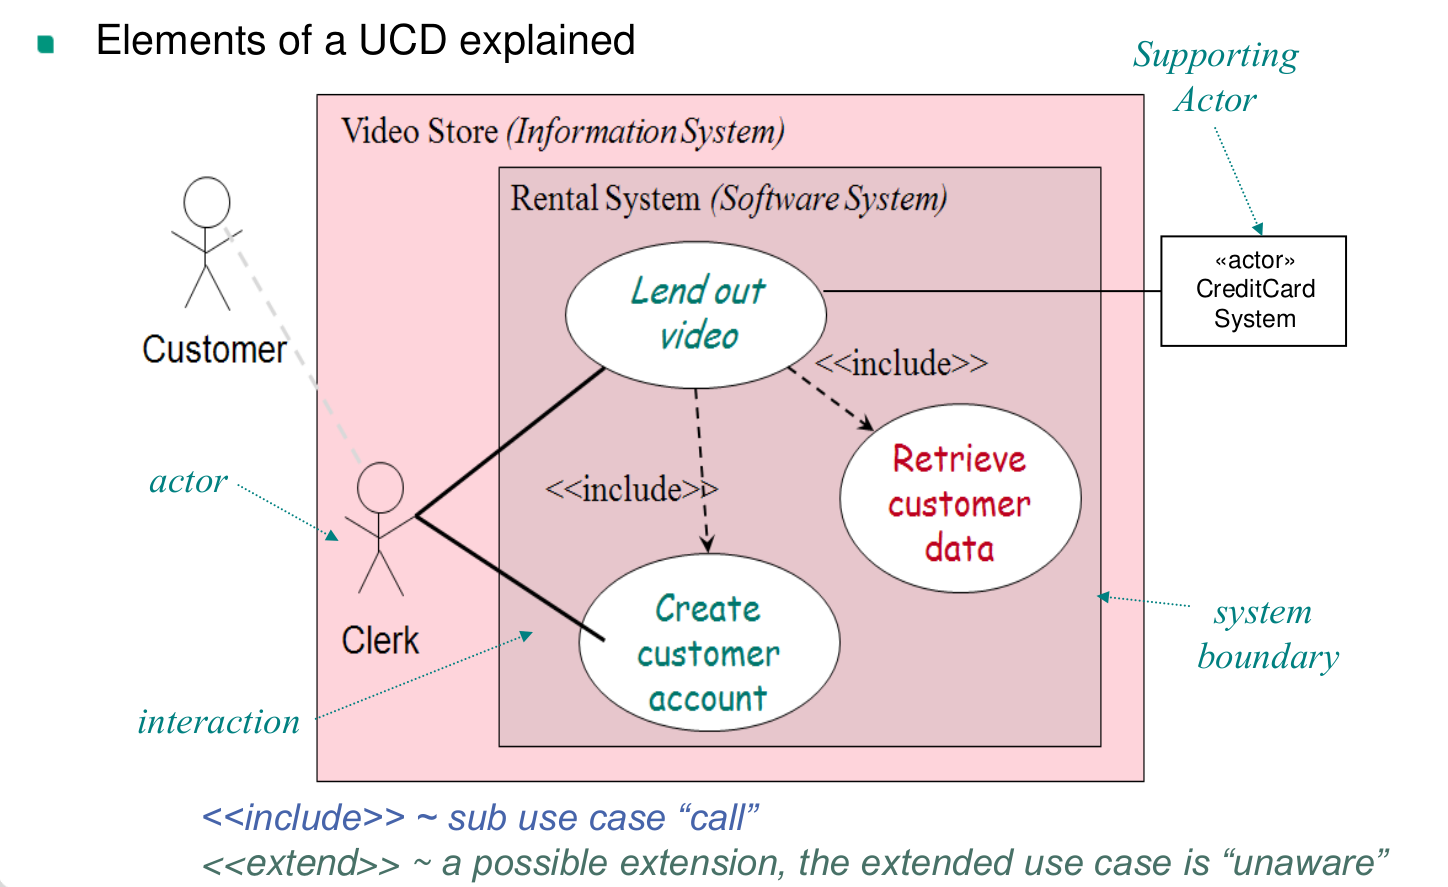
\includegraphics[width=0.85\textwidth]{images/usecase.png}
\end{figure}